\documentclass[a4paper]{article}

\usepackage[margin=1in]{geometry}
\usepackage{amsmath}
\usepackage{amssymb}
\usepackage{graphicx}
\usepackage{float}
\usepackage{hyperref}
\usepackage{caption}
\usepackage{subcaption}
\usepackage{amsfonts}
\usepackage{pdfpages}

\def\sectionautorefname{Section}
\def\subsectionautorefname{Section}
\def\subsubsectionautorefname{Section}
\def\figureautorefname{Figure}
\def\tableautorefname{Table}
\def\equationautorefname{Equation}


\begin{document}

%%%%%%%%%%%%%%%%%%%%%%%%%%
%%%%%%%%%%%%%%%%%%%%%%%%%%

\title{Random variables and random number generation}
\author{3F3 laboratory experiment \\ Theo A. Brown \\ Selwyn College, University of Cambridge}
\date{\today}
\maketitle

\tableofcontents

%%%%%%%%%%%%%%%%%%%%%%%%%%
%%%%%%%%%%%%%%%%%%%%%%%%%%

\section{Generating random numbers from the Uniform and Normal distributions}
\label{sec:uniform_normal}

%%%%%%%%%%%%%%%%%%%%%%%%%%

\subsection{Comparison of histogram with true probability density function}

A vector of Gaussian random numbers was generated using \verb`np.random.randn`, and a vector of uniformly distributed
random numbers generated using \verb`np.random.rand`. Histograms of the samples are plotted in
\autoref{fig:histogram_and_pdf}, overlaid with the exact probability density function (PDF). The histograms closely
follow the shape of the PDF, showing that the generation of the random numbers for these distributions is accurate.

\begin{figure}[h]
    \centering
    \begin{subfigure}[b]{0.45\textwidth}
        \centering
        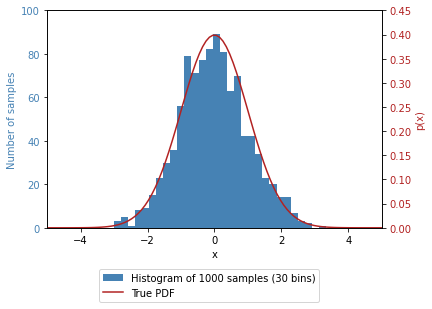
\includegraphics[width=\textwidth]{figures/gaussian_histogram_and_pdf.png}
        \caption{Gaussian distribution}
        \label{fig:gaussian_histogram_and_pdf}
    \end{subfigure}
    \hfill
    \begin{subfigure}[b]{0.45\textwidth}
        \centering
        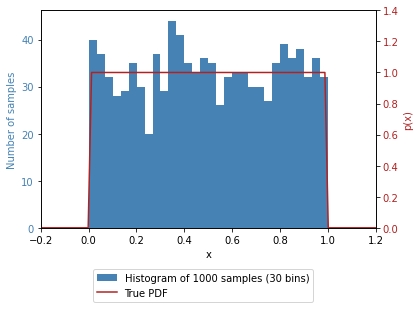
\includegraphics[width=\textwidth]{figures/uniform_histogram_and_pdf.png}
        \caption{Uniform distribution}
        \label{fig:uniform_histogram_and_pdf}
    \end{subfigure}
    \caption{Histogram of samples drawn from a distribution and true probability density function of distribution}
    \label{fig:histogram_and_pdf}
\end{figure}

%%%%%%%%%%%%%%%%%%%%%%%%%%

\subsection{Kernel density smoothing}

A smooth estimate of the probability density function is calculated using the kernel smoothing method with a Gaussian
kernel $\mathcal{N}(0, 1)$. The result is plotted for Gaussian and Uniform distributions in \autoref{fig:kernel_smoothed}.

\begin{figure}[h]
    \centering
    \begin{subfigure}[b]{0.45\textwidth}
        \centering
        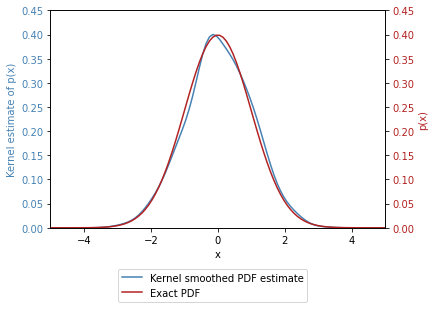
\includegraphics[width=\textwidth]{figures/gaussian_kernel_smoothed.png}
        \caption{Gaussian distribution}
        \label{fig:gaussian_kernel_smoothed}
    \end{subfigure}
    \hfill
    \begin{subfigure}[b]{0.45\textwidth}
        \centering
        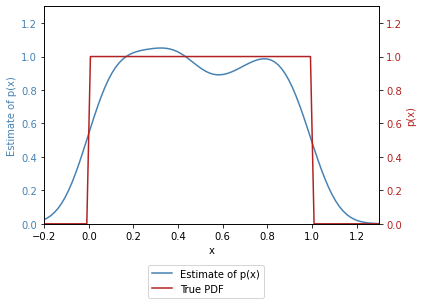
\includegraphics[width=\textwidth]{figures/uniform_kernel_smoothed.png}
        \caption{Uniform distribution}
        \label{fig:uniform_kernel_smoothed}
    \end{subfigure}
    \caption{Plot of true PDF and estimate of PDF generated using Gaussian kernel smoothing}
    \label{fig:kernel_smoothed}
\end{figure}

The kernel method takes an average of neighbouring values, weighted using a Gaussian distribution. This is advantageous
as it can smooth random irregularities in the samples: there may be histogram bins with a disproportionately high sample
count, which would give an incorrectly high estimate of the probability of this bin; the kernel smooths out this local
peak by taking neighbouring values into account. However, this also means that the kernel smoothing method becomes
inaccurate when there is a sudden change or discontinuity in the probability density function. In the Uniform
distribution there is zero probability for values outside the range $0<x<1$, but as the kernel averages over a window of
values it does not capture the step change at $x=0$ and $x=1$, instead decaying smoothly.

%%%%%%%%%%%%%%%%%%%%%%%%%%

\subsection{Multinomial distribution theory}

For N samples, let B be the random variable representing the number of samples in bin j. Let the probability that a
sample falls in bin j be $p_j$. By definition, the expected number of samples in bin j is $\mu_j = \mathbb{E}[B] = N p_j$,
and the variance in the number of samples in bin j is $\sigma^2_j = Var[B] = N p_j (1 - p_j)$.
\\
For the Uniform distribution between 0 and 1, the pdf $p(x)$ is defined as:
\begin{align*}
    p(x) &= \frac{1}{x_{max} - x_{min}} \\
         &= 1
\end{align*}
Hence, for a histogram with bin width $\delta$ and bin center $c_j$:
\begin{align*}
    p_j &= \int_{c_j - \delta/2}^{c_j + \delta/2}1\,dx \\
        &= \delta \\
    \mu_j &= N \delta \\
    \sigma_j &= \sqrt{N \delta (1 - \delta)}
\end{align*}
As $N$ becomes large, the estimate improves. The standard deviation increases less rapidly than the mean with increasing
$N$ ($\sigma \propto \sqrt{N}$ whereas $\mu \propto N$). Consequently an increase in $N$ will result in the standard
deviation becoming smaller compared to the mean ($\frac{\sigma}{\mu} \propto \frac{1}{\sqrt{N}}$). This is shown in
\autoref{fig:uniform_histogram_increasing_N}, where the standard deviation reduces as N increases.

\begin{figure}[h]
    \centering
    \begin{subfigure}[b]{0.3\textwidth}
        \centering
        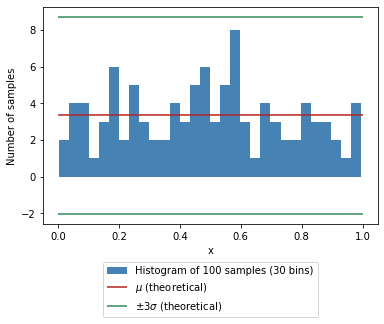
\includegraphics[width=\textwidth]{figures/uniform_histogram_100.png}
        \caption{$N=100$}
        \label{fig:uniform_histogram_100}
    \end{subfigure}
    \hfill
    \begin{subfigure}[b]{0.3\textwidth}
        \centering
        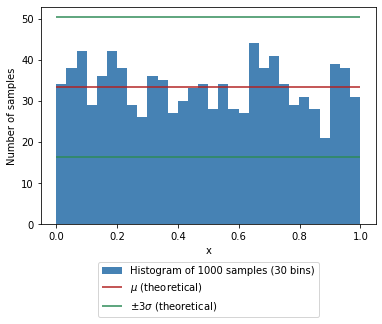
\includegraphics[width=\textwidth]{figures/uniform_histogram_1000.png}
        \caption{$N=1000$}
        \label{fig:uniform_histogram_1000}
    \end{subfigure}
    \hfill
    \begin{subfigure}[b]{0.3\textwidth}
        \centering
        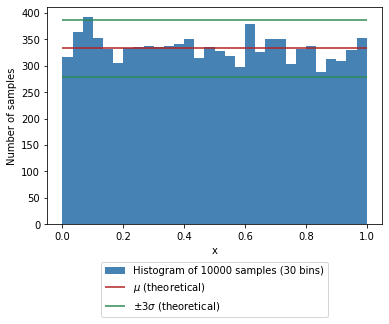
\includegraphics[width=\textwidth]{figures/uniform_histogram_10000.png}
        \caption{$N=10000$}
        \label{fig:uniform_histogram_10000}
    \end{subfigure}
    \caption{Histogram of uniformly distributed samples for increasing N, showing mean and $\pm3$ standard deviation}
    \label{fig:uniform_histogram_increasing_N}
\end{figure}

In \autoref{fig:uniform_histogram_increasing_N} it can be seen that the sample count lies within the $3\sigma$ interval
for all bins, so it is concluded that the results are consistent with the multinomial distribution theory.

%%%%%%%%%%%%%%%%%%%%%%%%%%
%%%%%%%%%%%%%%%%%%%%%%%%%%

\section{Functions of random variables}

\subsection{$f = a x + b$}
For $x \sim \mathcal{N}(0, 1)$, let $y = f(x) = a x + b$. Then:
\begin{align*}
    f^{-1}(y) &= \frac{y - b}{a} \\
    \left|\frac{dy}{dx}\right| &= |a| \\
    p_Y(y) &= \frac{1}{|a|} p_X \left( \frac{y - b}{a} \right) \\
    &= \frac{1}{|a|}\times\frac{1}{\sqrt{2\pi}} \exp{\left( -\frac{1}{2} \left( \frac{y-b}{a} \right)^2 \right)}
\end{align*}
Comparing with the equation for a general Gaussian distribution, it is clear that $p_Y(y)$ is a Gaussian distribution
with mean $b$ and variance $a$. This is shown in \autoref{fig:linear_function_of_gaussian}.

\begin{figure}[h]
    \centering
    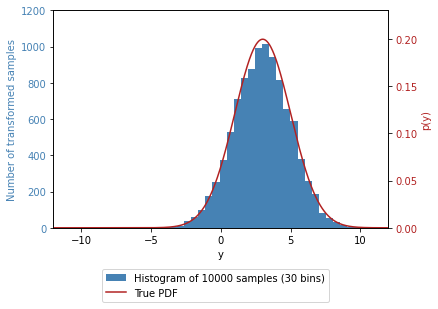
\includegraphics[width=0.6\textwidth]{figures/linear_function_of_gaussian.png}
    \caption{Histogram of linear function ($f(x^{(i)}) = 2x^{(i)} + 3$) of Gaussian samples overlaid with
    calculated PDF}
    \label{fig:linear_function_of_gaussian}
\end{figure}

%%%%%%%%%%%%%%%%%%%%%%%%%%

\subsection{$f = x^2$}
For $x \sim \mathcal{N}(0, 1)$, let $y = f(x) = x ^ 2$. Then:
\begin{align*}
    f^{-1}(y) &= \pm \sqrt{y} \\
    \left|\frac{dy}{dx}\right| &= |2x| \\
    p_Y(y) &= \sum_{i=1}^{2} \frac{1}{|2 \sqrt{y}|} p_X \left( \sqrt{y} \right) \\
    &= \frac{1}{\sqrt{2\pi y}} \exp{\left( -\frac{1}{2} y \right)}
\end{align*}

The result is plotted in \autoref{fig:quadratic_function_of_gaussian}.

\begin{figure}[h]
\centering
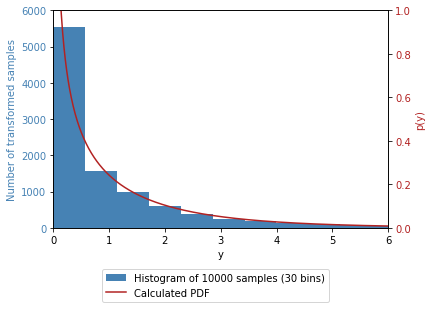
\includegraphics[width=0.6\textwidth]{figures/quadratic_function_of_gaussian.png}
\caption{Histogram of quadratic function $\left(f(x^{(i)}) = \left(x^{(i)}\right)^2\right)$) of Gaussian samples
overlaid with calculated PDF}
\label{fig:quadratic_function_of_gaussian}
\end{figure}

%%%%%%%%%%%%%%%%%%%%%%%%%%
%%%%%%%%%%%%%%%%%%%%%%%%%%

\section{Functions of random variables}

For the exponential distribution with mean one:
\begin{align*}
    & \text{PDF: } p(y) = \exp(-y), \ y \geq 0 \\
    & \text{CDF: } F(y) = \int_0^y p(y') dy' = 1 - \exp(-y) \\
    & \text{iCDF: } F^{-1}(x) = -\ln(1 - x)
\end{align*}

\autoref{fig:icdf_exponential} shows that samples from the exponential distribution generated using the iCDF follow the
true PDF.

\begin{figure}[h]
\centering
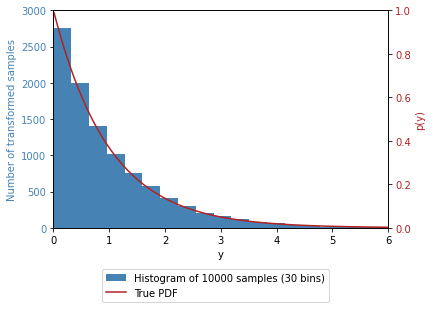
\includegraphics[width=0.6\textwidth]{figures/icdf_exponential.png}
\caption{Histogram of samples drawn from the uniform distribution and transformed using the iCDF method to follow the
exponential distribution, overlaid with the true exponential PDF}
\label{fig:icdf_exponential}
\end{figure}


%%%%%%%%%%%%%%%%%%%%%%%%%%
%%%%%%%%%%%%%%%%%%%%%%%%%%

\section{Simulation from non-standard densities}

Using the iCDF method, we can generate samples that are distributed according to:
\begin{align*}
    p(u) = \frac{\alpha^2}{2} \exp\left(-\frac{\alpha^2}{2} u\right)
\end{align*}
This distribution has:
\begin{align*}
    & \text{CDF: } F(u) = \int_0^u p(u') du' = 1 - \exp\left(-\frac{\alpha^2}{2} u\right) \\
    & \text{iCDF: } F^{-1}(v) = -\frac{2}{\alpha^2} \ln(1 - v)
\end{align*}
Samples $u^{(i)}$ can therefore be generated from uniformly distributed samples $v^(i)$.
The samples $u^{(i)}$ are then used to set the variance of the random variable X:
\begin{align*}
    p(x) = int_{0}^{\inf} \mathcal{N}(x\,|0, u) p(u) du
\end{align*}
The limit of the integral is from zero to infinity because the standard deviation must be positive.
A histogram of samples of $x^{(i)}$ is plotted in \autoref{fig:nonstandard_distribution} for different values of
$\alpha$. It appears that $\alpha$ sets the standard deviation of the distribution.
\begin{figure}[h]
\centering
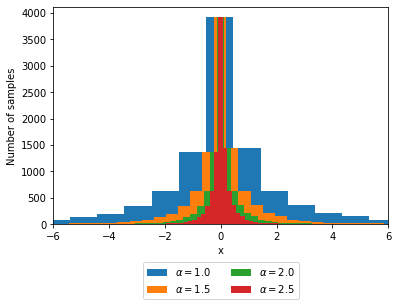
\includegraphics[width=0.6\textwidth]{figures/nonstandard_distribution.png}
\caption{100-bin histogram of samples drawn from the example distribution for different values of $\alpha$}
\label{fig:nonstandard_distribution}
\end{figure}

The kernel method was applied to the data, and the smoothed density was plotted on linear and log axes at different
scales (\autoref{fig:nonstandard_distribution_kernel_smoothed}). From the shape of the distribution
seems to be a sharper version of a Gaussian distribution, with significantly higher probability density in the centre
and tails that last for longer. Closer examination of the logarithmic plots suggests that the distribution behaves
more like a Gaussian close to $x=0$, where the logarithmic graph resembles an inverted parabola, and more like an
exponential further from $x=0$, where the logarithmic graph becomes linear.


\begin{figure}[h]
    \centering
    \begin{subfigure}[b]{0.3\textwidth}
        \centering
        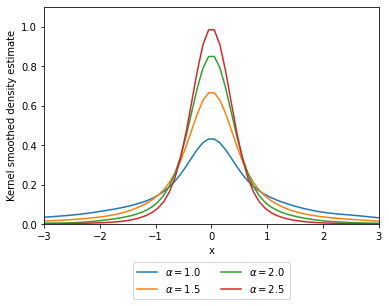
\includegraphics[width=\textwidth]{figures/nonstandard_distribution_ksdensity.png}
        \caption{Linear scale}
        \label{fig:nonstandard_distribution_kernel_smoothed_linear}
    \end{subfigure}
    \hfill
    \begin{subfigure}[b]{0.3\textwidth}
        \centering
        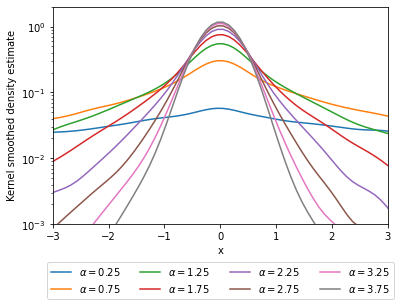
\includegraphics[width=\textwidth]{figures/nonstandard_distribution_ksdensity_log_close.png}
        \caption{$10^{-3} < \ln(p(x)) < 1$}
        \label{fig:nonstandard_distribution_ksdensity_log_close}
    \end{subfigure}
    \hfill
    \begin{subfigure}[b]{0.3\textwidth}
        \centering
        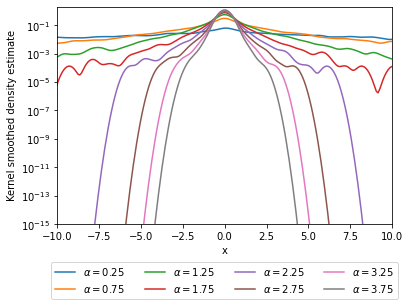
\includegraphics[width=\textwidth]{figures/nonstandard_distribution_ksdensity_log_far.png}
        \caption{$10^{-15} < \ln(p(x)) < 1$}
        \label{fig:nonstandard_distribution_ksdensity_log_far}
    \end{subfigure}
    \caption{Kernel smoothed probability density estimates for the example distribution}
    \label{fig:nonstandard_distribution_kernel_smoothed}
\end{figure}

%%%%%%%%%%%%%%%%%%%%%%%%%%
%%%%%%%%%%%%%%%%%%%%%%%%%%

\newpage
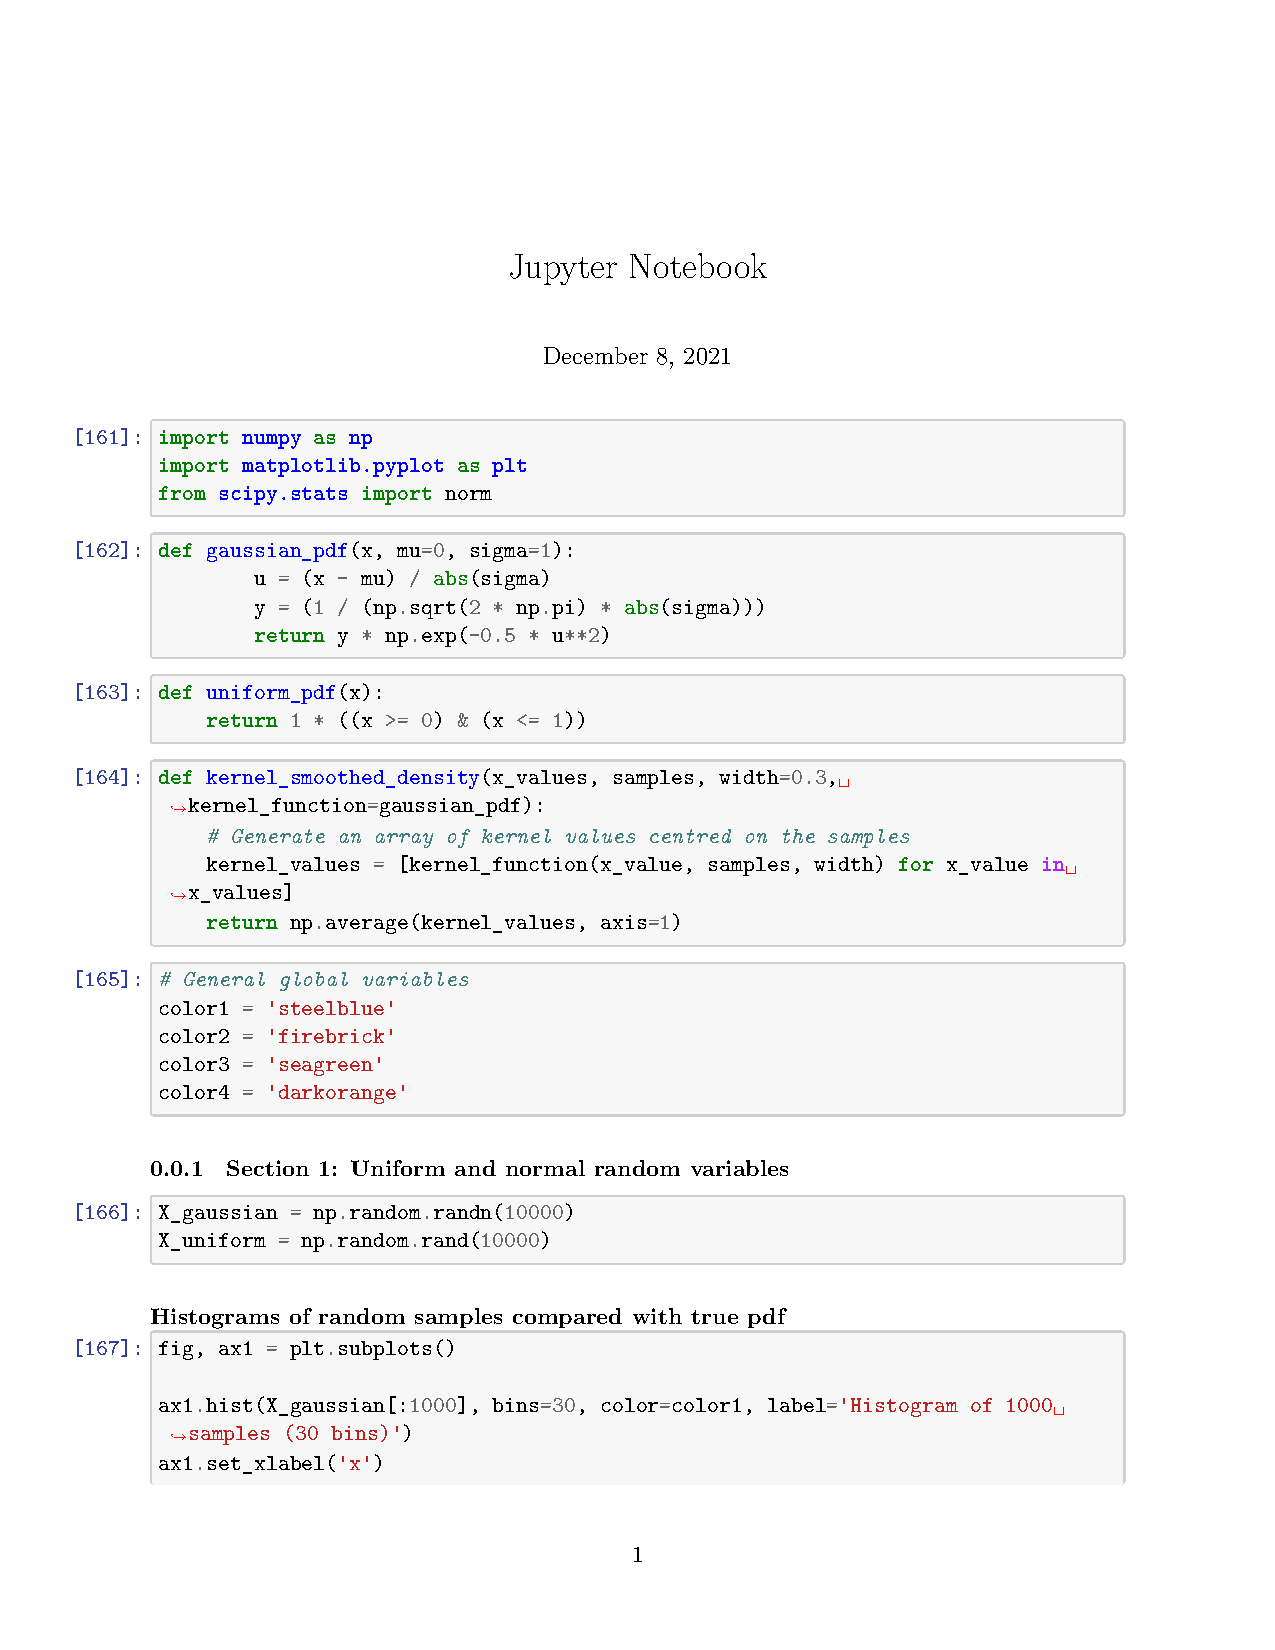
\includepdf[pages=-]{out/Jupyter Notebook.pdf}

\end{document}